\section{Werde zum Tennisspieler}
In dieser Aufgabe bauen wir ein kleines Tennisspiel, das auch unter dem Namen  \emph{Pong} bekannt ist. Ziel des Spieles ist es, einen Ball mit dem Schläger zu treffen. Verfehlt man den Schlag und trifft der Ball hinter einem auf den Rand, so erhält der Gegner einen Punkt. Wer als erster 10 Punkte erlangt hat, hat gewonnen.
\subsection{Programmiere einen Spieler}
Wir brauchen für das Spiel zwei Spieler. Beide verhalten sich gleich, daher reicht es einen Spieler zu malen und ihn im Anschluss zu kopieren. Wir erzeugen dazu ein weiteres Sprite.

\subsubsection{Male den Spieler}
\begin{enumerate}
\item Klicke auf das \textit{Neues Objekt malen}-Icon
\end{enumerate}
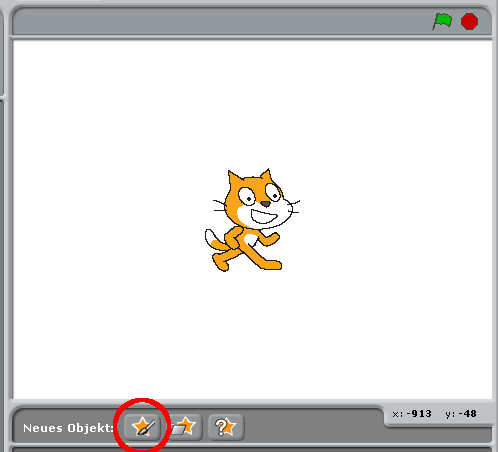
\includegraphics[width=0.6\textwidth]{images/aufgabe4_neues_objekt_malen.png}
\begin{enumerate}\addtocounter{enumi}{1}
\item Klicke auf das Quadrat, um das Rechteck-Tool auszuwählen.
\item Prüfe ob das ausgefüllte Quadrat unter den Werkzeugen selektiert ist.
\item Stelle sicher, dass die Farbe Schwarz ausgewählt ist
\item Zeichne nun durch gleichzeitiges Klicken und Ziehen mit der Maus ein Rechteck so wie es in folgendem Bild dargestellt ist.
\end{enumerate}
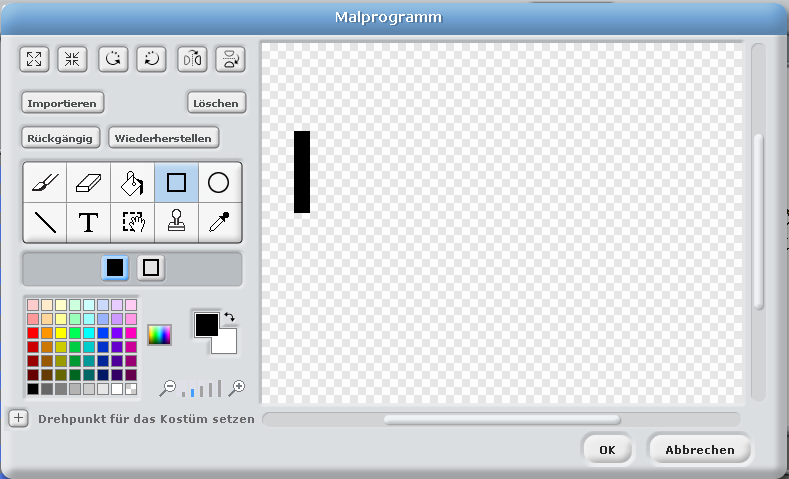
\includegraphics[width=0.6\textwidth]{images/aufgabe5_pong_sprite_spieler_malen.png}
\begin{enumerate}\addtocounter{enumi}{5}
\item Abschließend beende den Dialog durch betätigen der OK-Taste
\end{enumerate}
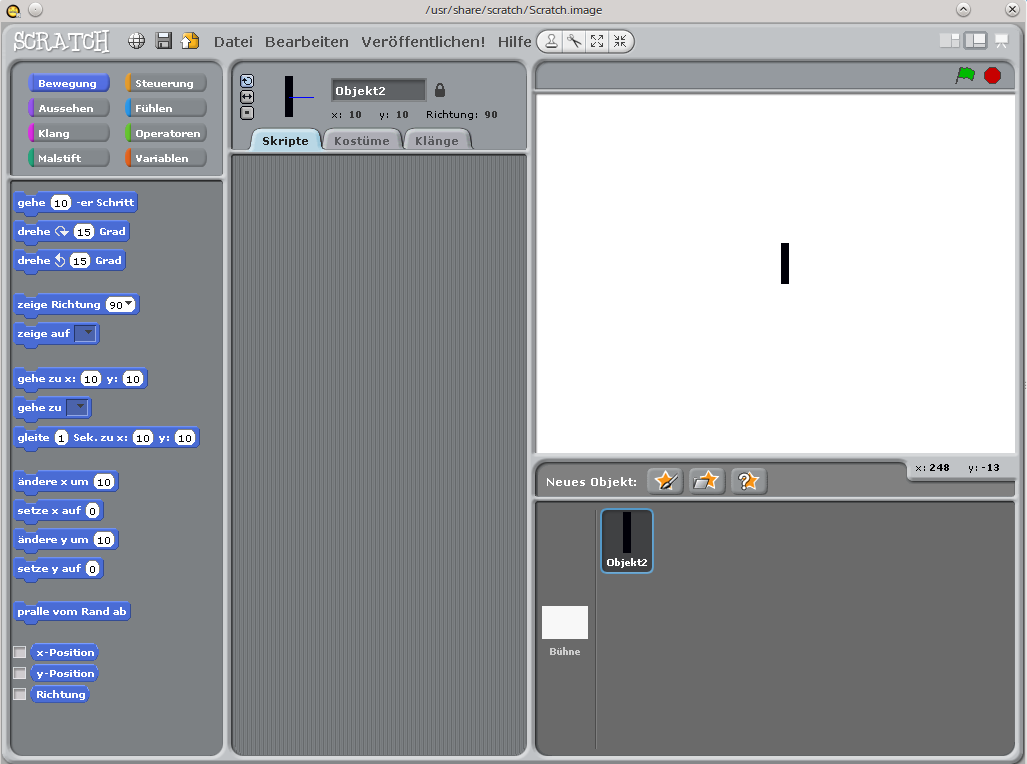
\includegraphics[width=0.6\textwidth]{images/aufgabe5_pong_sprite_spieler1_1.png}
\begin{enumerate}\addtocounter{enumi}{6}
\item Nun soll das neue Sprite noch den Namen \emph{Spieler1} erhalten
\item Als letztes lösche das Objekt mit der Katze, sofern es noch vorhanden ist
\end{enumerate}
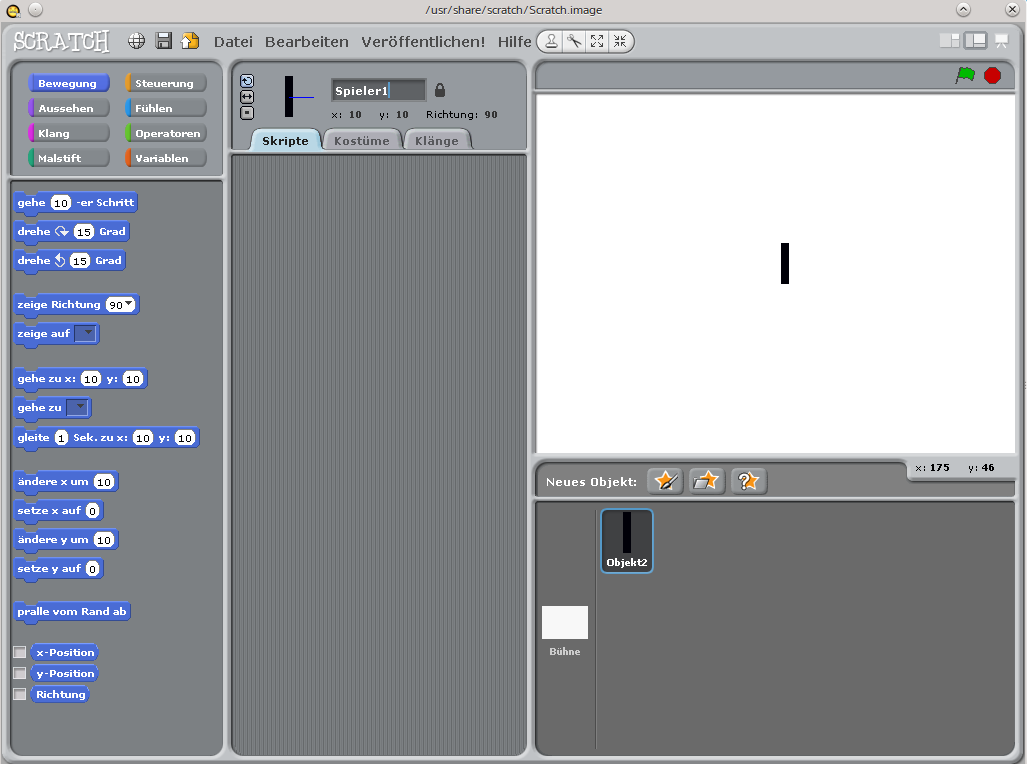
\includegraphics[width=0.6\textwidth]{images/aufgabe5_pong_sprite_spieler1_2.png}

\subsubsection{Programmiere das Verhalten des Spielers}

Nachdem nun der Spieler gemalt wurde muss sein Verhalten programmiert werden: Der Spieler soll durch betätigen der Taste \emph{w} nach oben und durch betätigen der Taste \emph{s} nach unten bewegt werden können.


\begin{enumerate}
\item Klicke auf den Sprite \emph{Spieler1}.
\item Für die Bewegung nach oben ziehe folgende Kacheln in dein Skript-Panel:
  \begin{enumerate}
  \item Aus dem Steuerungs-Panel die Kachel \textit{Wenn Taste Leertaste gedrückt} und \textit{wiederhole fortlaufend} und setze sie zusammen.
  \item Füge nun aus dem Steuerungs-Panel die Kachel \textit{warte bis} in die Schleife ein.
  \item Aus dem Fühlen-Panel die Kachel \textit{Taste ... gedrückt?}. Diese Kachel setzt du als Bedingung in die \textit{warte bis}-Kachel und wählst als Taste \emph{w} aus 
  \item Aus dem Bewegung-Panel suchst du die Kachel \textit{ändere y um ...} raus und fügst diese unter die Bedingung \textit{warte bis} ein. Setze den Wert in der Kachel auf \emph{10}    
  \end{enumerate}
\item Für die Bewegung nach unten dupliziere nun die eben angelegten Anweisungen und passe diese an:
  \begin{enumerate}
  \item passe die Kachel \textit{warte bis}-Kachel so an, dass auf die Taste \emph{s} gewartet wird
  \item ändere die Kachel \textit{ändere y um ...} auf \emph{-10}  
  \end{enumerate}
\item Damit der Spieler immer an der richtigen Stelle startet, ziehe folgende Kacheln in dein Skript-Panel:
  \begin{enumerate}
  \item Aus dem Steuerungs-Panel die Kachel \textit{Wenn Taste Leertaste gedrückt}
  \item Aus dem Aussehen-Panel die Kachel \textit{zeige dich} und füge sie an \textit{Wenn Taste Leertaste gedrückt}
  \item Aus dem Bewegung-Panel die Kachel \textit{gehe zu x: ... y: ...}, fügst diese an die Kachel \textit{zeige dich} und trägst für \emph{x} \emph{-200} und für \emph{y} \emph{0} ein.
  \end{enumerate}
\end{enumerate}

Damit ist der erste Spieler fertig. Dein Programm sollte nun so aussehen:

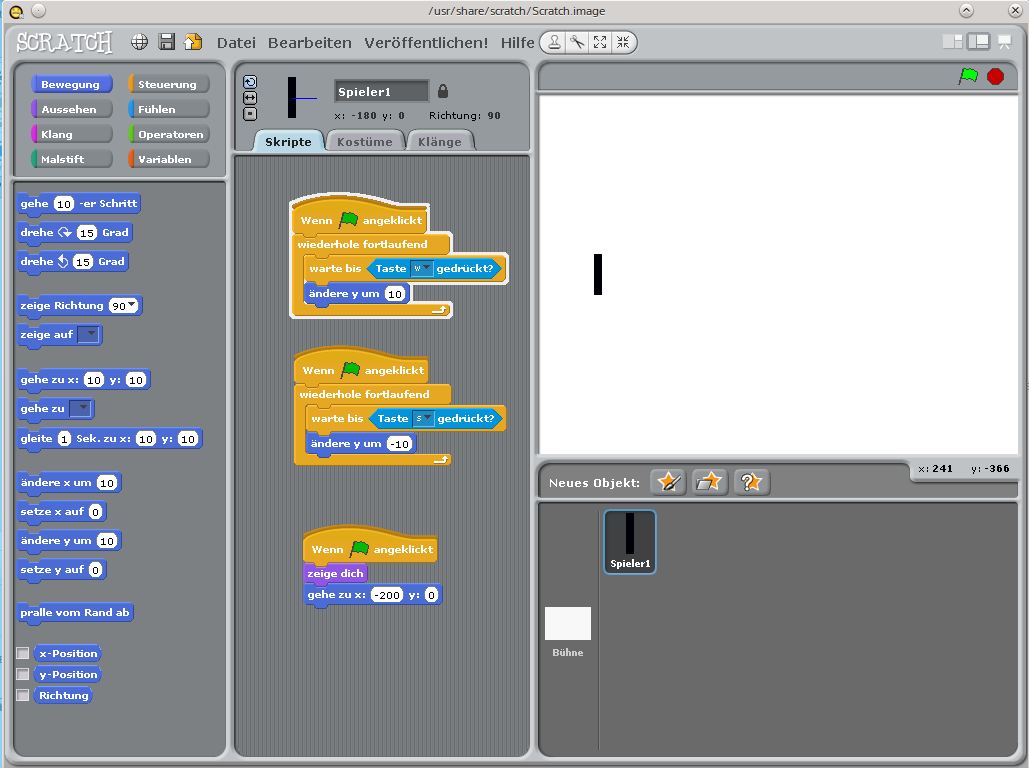
\includegraphics[width=1\textwidth]{images/aufgabe5_pong_sprite_spieler1_3.png}

Probiere ob du deinen Spieler mit den Tasten \emph{w} und \emph{s} steuern kannst.

\subsubsection{nun der zweite Spieler}

Den zweiten Spieler können wir durch kopieren des ersten erstellen. Anschließend müssen wir nur noch die Position auf dem Spielfeld und die Tasten für die Bewegung anpassen.

\begin{enumerate}
\item Wähle den Sprite \emph{Spieler1} und dupliziere ihn über den Menüeintrag im Kontextmenü (Das Menü erscheint, wenn du die rechte Maustaste auf dem Sprite betätigst)
\item Selektiere nun das neu erstellt Sprite und ändere seinen Namen auf \emph{Spieler2}
\item Ändere nun in der Kachel \textit{Taste w gedrückt?} die Taste auf \emph{o}
\item In der Kachel \textit{Taste s gedrückt?} änderst du die Taste auf \emph{l}
\item Abschließend ändere die \emph{x}-Position in der Kachel \textit{gehe zu x: -200 y: 0} auf \emph{200}
\end{enumerate}

Der zweite Spieler sollte nun so aussehen:

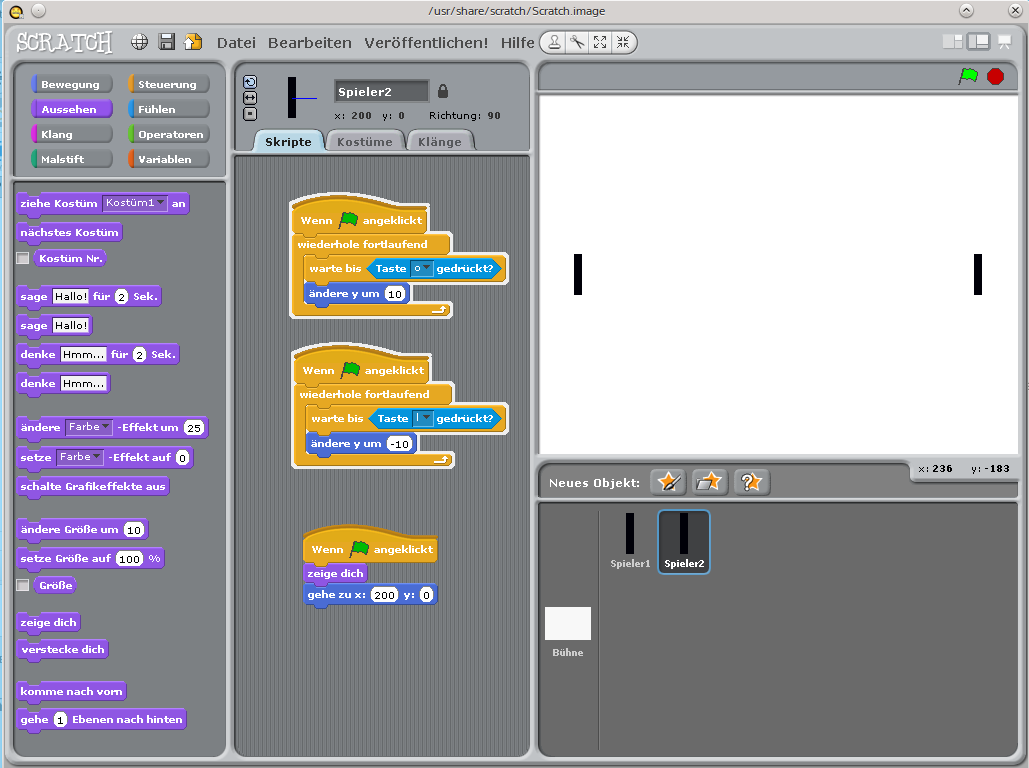
\includegraphics[width=1\textwidth]{images/aufgabe5_pong_sprite_spieler2.png}

Probiere aus, ob du beide Spieler mit den Tasten \emph{w,s} und \emph{o,l} bedienen kannst.

\subsection{Der Ball kommt ins Spiel}
Nun muss das Verhalten des Balls programmiert werden: Der Ball soll vom Rand abprallen. Wenn ein Spieler den Ball trifft, soll der Ball zurückgeschlagen werden. Trifft der Ball hinter einem Spieler auf den Rand, erhält der andere Spieler einen Punkt.

\subsubsection{Male einen Ball}
Zunächst klicke auf das \textit{Neues Objekt malen}-Icon, um einen Sprite für den Ball zu erzeugen. 
Du malst einen Ball mit Hilfe des Werkzeugs \emph{Ellipse}:

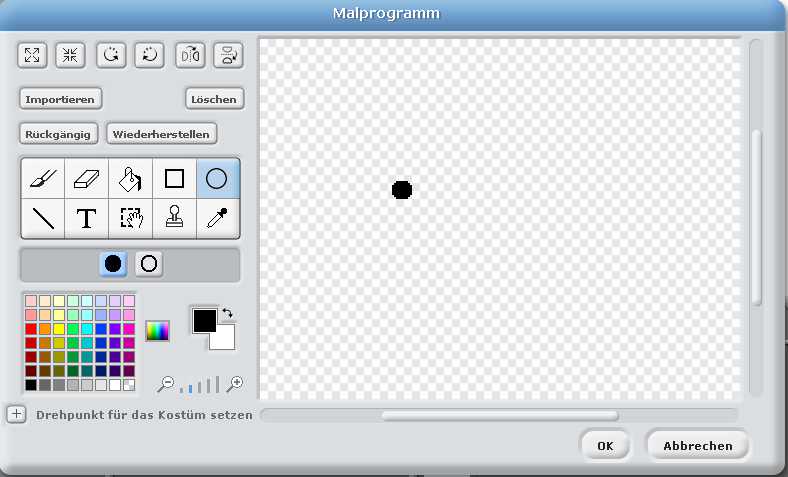
\includegraphics[width=0.6\textwidth]{images/aufgabe5_pong_sprite_ball_malen.png}


\subsubsection{Der Ball fliegt}
\begin{enumerate}
\item Selektiere nun das neu erstellt Sprite und ändere seinen Namen auf \emph{Ball}.
\item Füge nun die Kachel \textit{Wenn grüne Fahne angeklickt} dem Skript für den Ball zu.
\item Als nächsten initialisiere  den Ball. 
Initialisieren bedeutet, beim Programmstart Dinge festzulegen, damit das Programm immer gleich abläuft. In unserem Fall bedeutet dies, beim Spielstart eine Ausgangssituation für den Ball festzulegen. So startet der Ball immer an der gleichen Position:
\begin{enumerate}
\item Füge die Kachel \textit{zeige dich} an die Kachel \textit{Wenn grüne Fahne angeklickt}
\item Als nächsten Befehl füge die Kachel \textit{gehe zu x: y:} an die Kachel \textit{zeige dich}. Setze den Wert für \emph{x} auf \emph{-200} und für \emph{y} auf \emph{0}
\item Zum Spielbeginn soll der Ball in eine zufällige Richtung fliegen. Dies erreichst du indem, du die Kachel \textit{zeige Richtung} verwendest und als Wert die Kachel \textit{Zufallszahl von: bis:} einfügst. Trage für \emph{von} \emph{50} und für \emph{bis} \emph{130} ein.
\item Füge die Kachel \textit{zeige Richtung} nun an die Kachel  \textit{gehe zu x: y:} an.
\end{enumerate}
\item Nach der Initialisierung kann nun der Ball zum Programmstart in eine zufällige Richtung zeigen, aber sich noch nicht bewegen. Das ist noch kein richtiges Spiel, daher sollen die nun folgenden Anweisungen immer wieder ausgeführt werden. Das erreichst du indem du die Kachel \textit{wiederhole fortlaufend} an die letzte Kachel deines Skripts anfügst. 
\item Nun kommen die Dinge, die der Ball immer wieder ausführen soll:
\begin{enumerate}
\item Als erstes soll der Ball von der Wand abprallen, wenn er sie berührt. Dazu ziehst du die Kachel \textit{pralle von Rand ab} in die Schleife \textit{wiederhole fortlaufend}. 
\item Damit sich der Ball bewegt, fügst du die Kachel \textit{gehe ... er Schritt} an die Kachel \textit{pralle von Rand ab}. Setze den Wert in der Kachel auf \emph{10}. Dieser Wert bestimmt wie schnell der Ball fliegt.  
\item Jetzt fehlt noch das Schlagen des Balls durch die Spieler. Durch den Schlag ändert der Ball zufällig seine Richtung:
\begin{enumerate}
\item Füge die Kachel \textit{falls} an die letzte Kachel in der Schleife ein.
\item Verwende als Bedingung für die Kachel \textit{wird ... berührt?} und wähle aus der Liste der Objekte dafür \emph{Spieler1}
\item Füge nun in die Kachel \textit{falls} die Kachel \textit{zeige Richtung ...} ein.
\item Als Wert für die Richtung verwendest du die Kachel \textit{Zufallszahl von: bis:}.
\item Trage für \emph{von} \emph{50} und für \emph{bis} \emph{130} ein.
\end{enumerate}
\item Tue das Gleiche für den zweiten Spieler.
\item Für den zweiten Spieler muss der Wertebereich für die Zufallszahl \emph{von} \emph{-50}  \emph{bis} \emph{-130} gehen. 
\end{enumerate}
\end{enumerate}

So sollte dein Skript jetzt aussehen: 

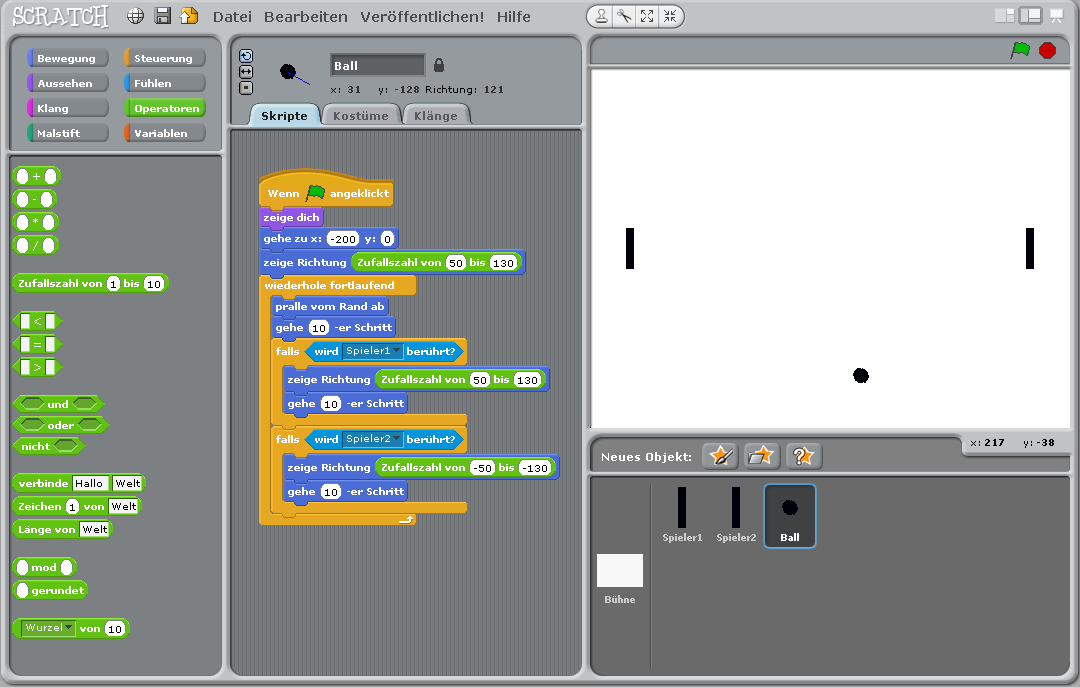
\includegraphics[width=1\textwidth]{images/aufgabe5_pong_sprite_ball_1.png}


\subsection{Der Hintergrund}
Nun soll der Hintergrund verändert werden. Zum einen soll der Hintergrund um Auslinien erweitert werden. Berührt der Ball diese so erhält ein Spieler einen Punkt. Ferner sollen zwei weitere Hintergründe gemalt werden: Einen der anzeigt, dass \textit{Spieler 1} gewonnen hat und  einen  der anzeigt, dass \textit{Spieler 2} gewonnen hat.

\begin{enumerate}
\item Selektiere die Bühne und wähle anschließend die Registerkarte \textit{Hintergründe}
\item Klicke nun für den \textit{Hintergrund 1} die Schaltfläche \textit{bearbeiten}
\item Füge auf der linken Seite des Hintergrunds mit dem Werkzeug \textit{Rechteck} eine rote Linie ein 
\item Füge auf der rechten Seite des Hintergrunds mit dem Werkzeug \textit{Rechteck} eine blaue Linie ein
\item Schließe den Dialog mit \textit{ok}
\end{enumerate}

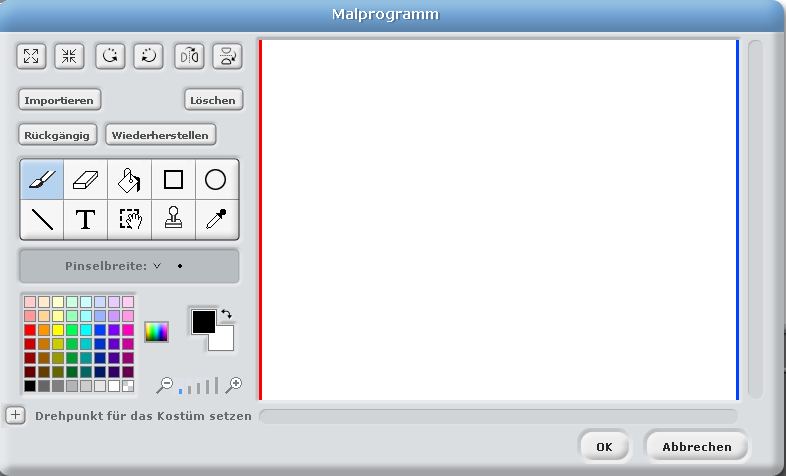
\includegraphics[width=0.6\textwidth]{images/aufgabe5_pong_hintergrund_malen.png}

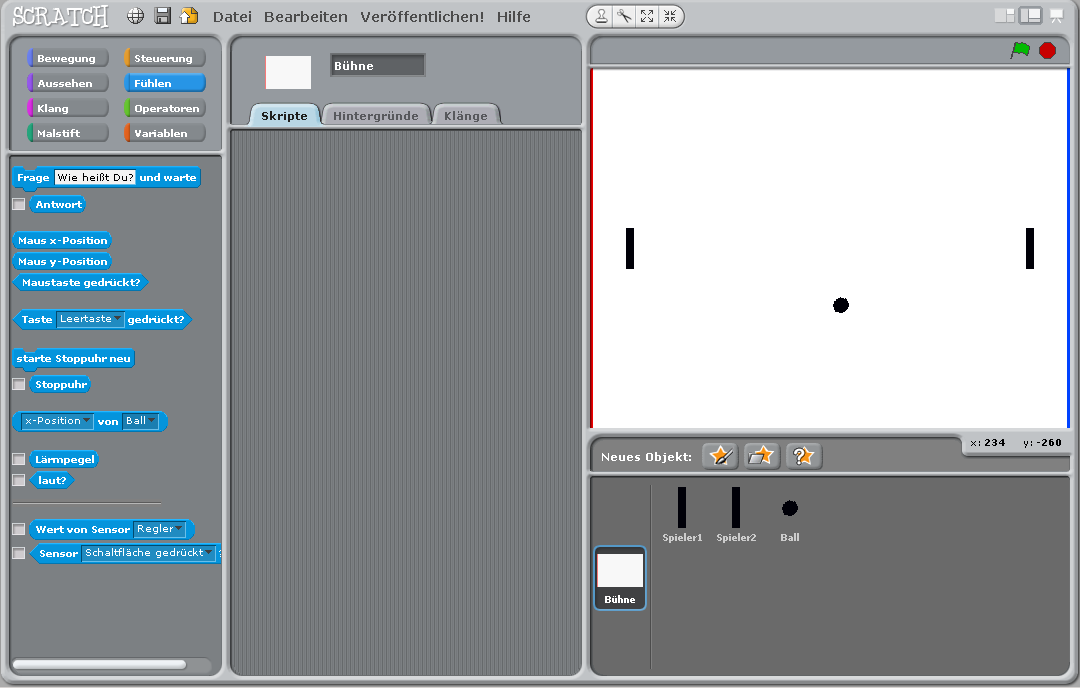
\includegraphics[width=0.6\textwidth]{images/aufgabe5_pong_hintergrund_1.png}


\begin{enumerate}\addtocounter{enumi}{5}
\item Nun klicke auf der Registerkarte \textit{Hintergründe} die Schaltfläche \textit{male}
\item Verwende das Werkzeug \textit{Text} 
\item Schreibe den Text \textit{Spieler 1 hat gewonnen}
\item Schließe den Dialog mit \textit{ok}
\item Benenne diesen Hintergrund \textit{Spieler1HatGewonnen}
\end{enumerate}

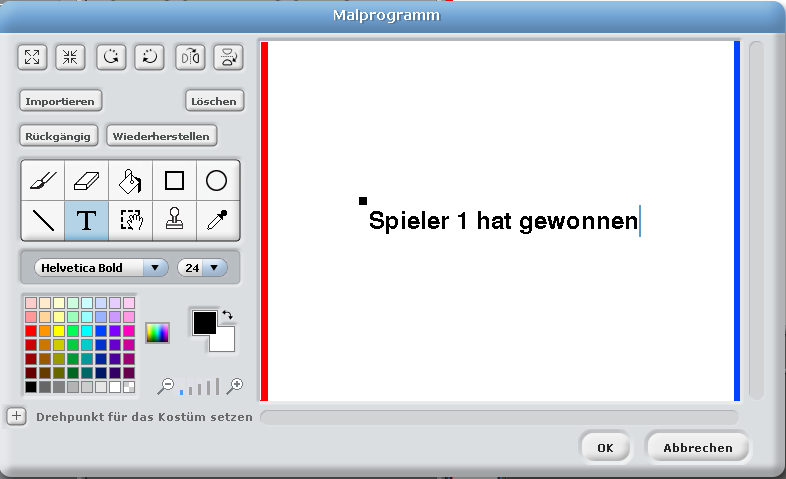
\includegraphics[width=0.6\textwidth]{images/aufgabe5_pong_hintergrund_gewonnen_malen.png}

Wiederhole die letzten Schritte, um einen weiteren Hintergrund mit dem Text \textit{Spieler 2 hat gewonnen} anzulegen. Nenne diesen Hintergrund \textit{Spieler2HatGewonnen}. Das Endergebnis sieht nun so aus:

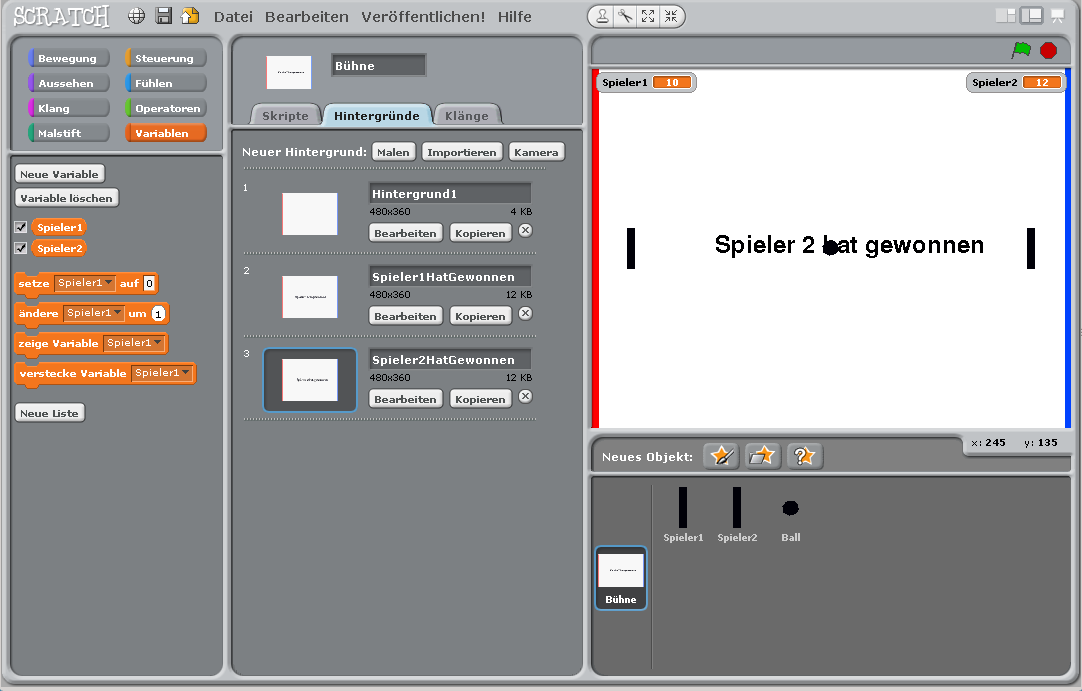
\includegraphics[width=1\textwidth]{images/aufgabe5_pong_hintergrund_2.png}



\subsection{Wer hat gewonnen?}
Als letzten Schritt soll der Spielstand gezählt werden. Der Spieler, der als erster 10 Punkte erzielt, hat gewonnen. 
Dafür müssen wir für jeden Spieler eine Variable anlegen. 
Variablen ermöglichen einen Wert hinein zu schreiben und zu einem späteren Zeitpunkt diesen Wert wieder auszulesen. Dies ist vergleichbar mit einer Tasche in die man ein Teil legt und später wieder herausnehmen oder einfach nur nachsehen kann, welches Teil in der Tasche ist. 

\begin{enumerate}
\item Klicke im Bereich Variablen auf die Schaltfläche \textit{Neue Variable}
\item Benenne in dem sich öffnenden Dialog die Variable \textit{Spieler1} und schließe den Dialog mit \textit{Ok}
\item Klicke nun nochmals auf die Schaltfläche \textit{Neue Variable}
\item Benenne diesmal die Variable \textit{Spieler2} und schließe den Dialog mit \textit{Ok}
\item Du kannst mit der Maus die Position der Variablen auf der Bühne verändern
\end{enumerate}

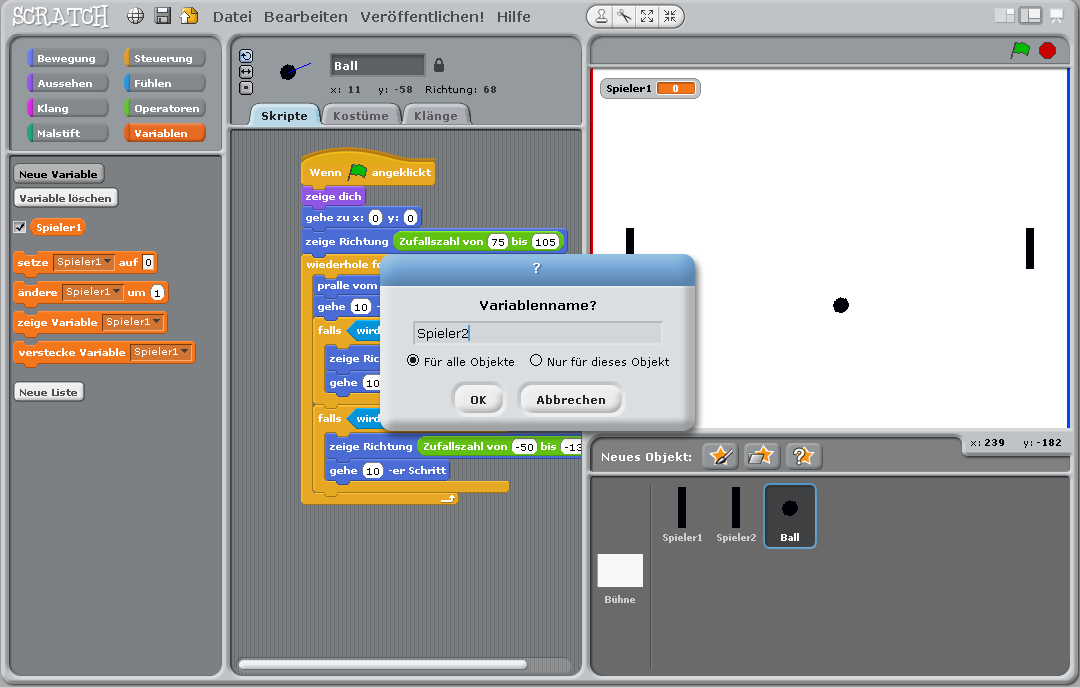
\includegraphics[width=1\textwidth]{images/aufgabe5_pong_spieler_variablen_1.png}

Nun müssen die Variablen zum Spielbeginn mit \emph{0} initialisiert und immer dann hochgezählt werden, wenn der Ball die Auslinien berührt: 
\begin{enumerate}\addtocounter{enumi}{5}
\item Füge zum Skript des Balls eine weitere Kachel \textit{Wenn grüne Fahne angeklickt} ein
\item Füge an diese Kachel aus dem Bereich Variablen die Kachel \textit{setze ... auf ...} 
\item wähle aus der Liste dieser Kachel die Variable \textit{Spieler1}  und setze den Wert auf \emph{0}
\item füge an diese Kachel erneut eine Kachel \textit{setze ... auf ...} 
\item wähle dieses Mal die Variable \textit{Spieler2},  setze den Wert ebenfalls auf \emph{0}
\item Nun wird in einer Schleife geprüft, ob die Auslinien berührt werden. Füge dazu die Kachel \textit{wiederhole fortlaufend} an die letze Kachel
\item Innerhalb der Schleife füge nun  zunächst eine Kachel \textit{falls} ein
\item Als Bedingung dieser Kachel wähle die Kachel \textit{wird Farbe ... berührt?} 
\item Die zu prüfende Farbe ist in diesem Fall \textit{blau}
\item Innerhalb der Kachel \textit{falls} füge eine Kachel \textit{ändere ... um ...} und wähle für diese Kachel die Variable \textit{Spieler1} aus der Liste. Als Wert für \emph{um} setze \emph{1} 
\item Nachdem ein Ball im Aus landet, muss der Spieler erneut mit zufälliger Richtung abschlagen. Füge an die Kachel für die Erhöhung der Variable eine Kachel \textit{zeige Richtung ...}. Als Wert wähle mithilfe der Kachel \textit{Zufallszahl von ... bis ...}  eine Zufallszahl im Bereich \emph{-50} bis \emph{-130}
\item Lasse an diese Kachel eine Kachel \textit{gehe zu x: ... y: ...} folgen und setze für \emph{x} den Wert \emph{200} und für \emph{y} den Wert \emph{0} ein
\item Dupliziere nun die \textit{falls}-Kachel mit den enthaltenen Anweisungen und passe diese an:
\begin{enumerate}
\item Ändere in der Kopie die Farbe in der Bedingung auf \emph{rot}
\item Wechsel die zu erhöhende Variable auf \textit{Spieler2}
\item Erzeuge die Zufallszahlen in dem Bereich \emph{50} bis \emph{130}
\item Abschließend trage für den \emph{x}-Wert der \textit{gehe zu x: ... y: ...} Kachel den Wert \emph{200} ein
\end{enumerate}
\end{enumerate}


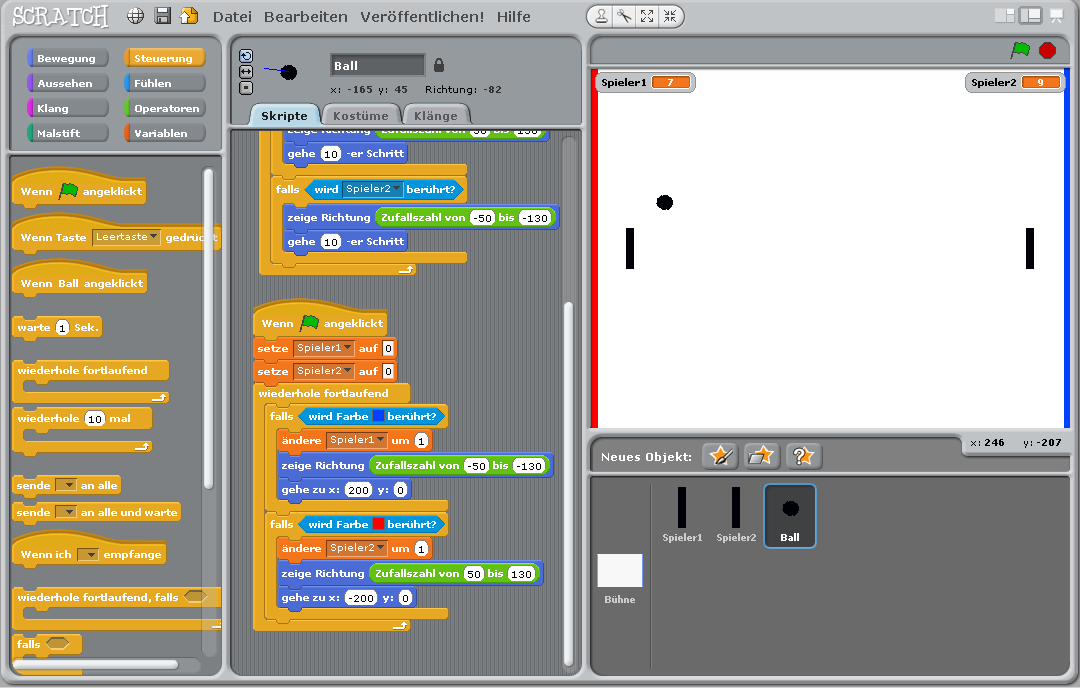
\includegraphics[width=1\textwidth]{images/aufgabe5_pong_spieler_variablen_2.png}


Soweit so gut! Nun muss das Spiel nur noch enden, wenn ein Spieler 10 Punkte erreicht. Wenn dies geschieht soll der Hintergrund so gewechselt werden, dass der Spieler angezeigt wird, der gewonnen hat. 
Du erreichst dies, indem du ein Skript für den Hintergrund erstellst. Dieses initialisiert den Hintergrund bei Spielstart und wechselt diesen sobald ein Spieler 10 Punkte erreicht:

\begin{enumerate}\addtocounter{enumi}{18}
\item Wähle die Bühne und füge dem Skript-Register die Kachel \textit{Wenn grüne Fahne angeklickt} ein
\item Füge an diese Kachel die Kachel \textit{wechsle zu ...} ein und wähle in der Liste den \emph{Hintergrund1}
\item Nun füge erneut die Kachel \textit{Wenn grüne Fahne angeklickt} ein
\item Füge an diese eine Schleife mittels der Kachel \textit{wiederhole fortlaufend}
\item In die Schleife fügst du nun eine Kachel \textit{falls}. 
\item Als Bedingung fügst du nun die Operatorkachel \textit{=} ein. Den einen Wert des Operators setzt du auf \emph{10} für den anderen verwendest du die Variable \textit{Spieler1}. Hierdurch wird der \textit{falls}-Block nur betreten, wenn die Variable \textit{Spieler1} den Wert \emph{10} besitzt
\item In den \textit{falls}-Block fügst du nun die Kachel \textit{wechsle zu ...} ein und wähle in der Liste den Hintergrund \emph{Spieler1HatGewonnen}
\item Füge an diese Kachel die Kachel \textit{stoppe alles, um das Spiel anzuhalten}
\item Dupliziere nun den gesamten Block ab der Kachel \textit{Wenn grüne Fahne angeklickt} 
\item Verwende in dem neuen Block in der \textit{falls}-Bedingung die Variable \textit{Spieler2}
\item Passe im  \textit{falls}-Block den anzuzeigenden Hintergrund an, so dass der Hintergrund \textit{Spieler2HatGewonnen} angezeigt wird.
\end{enumerate}

Dein fertiges Skript sollte nun so aussehen: 

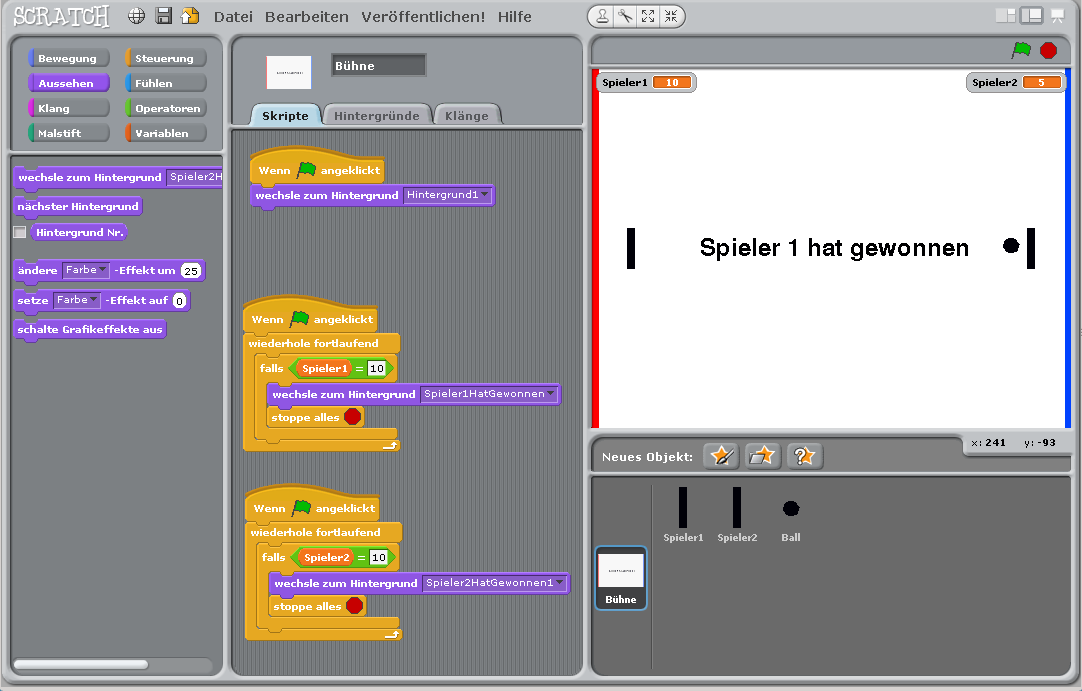
\includegraphics[width=1\textwidth]{images/aufgabe5_pong_spieler_variablen_3.png}

Nun ist es Zeit das Spiel auszuprobieren.

\subsection{Erweiterungen}
Das Pong-Spiel ist nun fertig; dennoch kannst du es erweitern:

\begin{enumerate}
\item Versuche das Programm so zu erweitern, dass der Ball schneller wird sobald ein Spieler den Ball getroffen hat. Du brauchst dafür eine weitere Variable, die die Geschwindigkeit des Balls enthält.
\item Die Auslinien sind durch die rote und blaue Linie im Hintergrund dargestellt. Gezählt wird, wenn der Ball die rote oder blaue Farbe berührt. Überlege, wie du das Programm umbauen müsstest, wenn die Auslinien selbst Objekte sind. Diese Objekte sollen merken können sobald sie der Ball trifft und die Punkte entsprechend anpassen.
\item Nachdem die Auslinien Objekte geworden sind, kannst du aus dem Tennisspiel ein Fußballspiel machen. Hierzu brauchst du nur die Auslinien auf Torlänge zu kürzen. 
\end{enumerate}








